\documentclass{beamer}

\mode<presentation> {

  % The Beamer class comes with a number of default slide themes
  % which change the colors and layouts of slides. Below this is a list
  % of all the themes, uncomment each in turn to see what they look like.

  %\usetheme{default}
  %\usetheme{AnnArbor}
  %\usetheme{Antibes}
  %\usetheme{Bergen}
  %\usetheme{Berkeley}
  %\usetheme{Berlin}
  %\usetheme{Boadilla}
  %\usetheme{CambridgeUS}
  %\usetheme{Copenhagen}
  %\usetheme{Darmstadt}
  %\usetheme{Dresden}
  %\usetheme{Frankfurt}
  %\usetheme{Goettingen}
  %\usetheme{Hannover}
  %\usetheme{Ilmenau}
  %\usetheme{JuanLesPins}
  %\usetheme{Luebeck}
  \usetheme{Madrid}
  %\usetheme{Malmoe}
  %\usetheme{Marburg}
  %\usetheme{Montpellier}
  %\usetheme{PaloAlto}
  %\usetheme{Pittsburgh}
  %\usetheme{Rochester}
  %\usetheme{Singapore}
  %\usetheme{Szeged}
  %\usetheme{Warsaw}


  %\usecolortheme{albatross}
  %\usecolortheme{beaver}
  %\usecolortheme{beetle}
  %\usecolortheme{crane}
  %\usecolortheme{dolphin}
  %\usecolortheme{dove}
  %\usecolortheme{fly}
  %\usecolortheme{lily}
  %\usecolortheme{orchid}
  %\usecolortheme{rose}
  %\usecolortheme{seagull}
  %\usecolortheme{seahorse}
  %\usecolortheme{whale}
  %\usecolortheme{wolverine}
}

\usepackage{graphicx} 
\usepackage{booktabs} 
\usepackage{hyperref}
\usepackage{caption}
\usepackage{subfig}
\usepackage{subcaption}

\captionsetup[subfigure]{labelformat=empty}
\captionsetup[figure]{labelformat=empty}
\graphicspath{{./graphics/}}

\AtBeginSection[]
  {
     \begin{frame}<beamer>
     \frametitle{Outline}
     \tableofcontents[currentsection]
     \end{frame}
  }
%----------------------------------------------------------------------------------------
%       TITLE PAGE
%----------------------------------------------------------------------------------------

\title[Vim workshop]{Vim workshop} 

\author{Joan V. and Guillem R.}
\institute[LinuxUPC]
{
  LinuxUPC \\
  \medskip
  \textit{linuxupc AT linuxupc.upc.edu} 
}
\date{\today} 

\begin{document}

\begin{frame}
  \titlepage
\end{frame}

\begin{frame}
  \frametitle{Outline} 
  \tableofcontents 
\end{frame}

%----------------------------------------------------------------------------------------
%       PRESENTATION SLIDES
%----------------------------------------------------------------------------------------
%------------------------------------------------
\section{Background}
%------------------------------------------------
\subsection{Exiting Vim}
\begin{frame}{Exiting Vim}
\begin{figure}[htp] 
    \centering
    \subfloat{%
        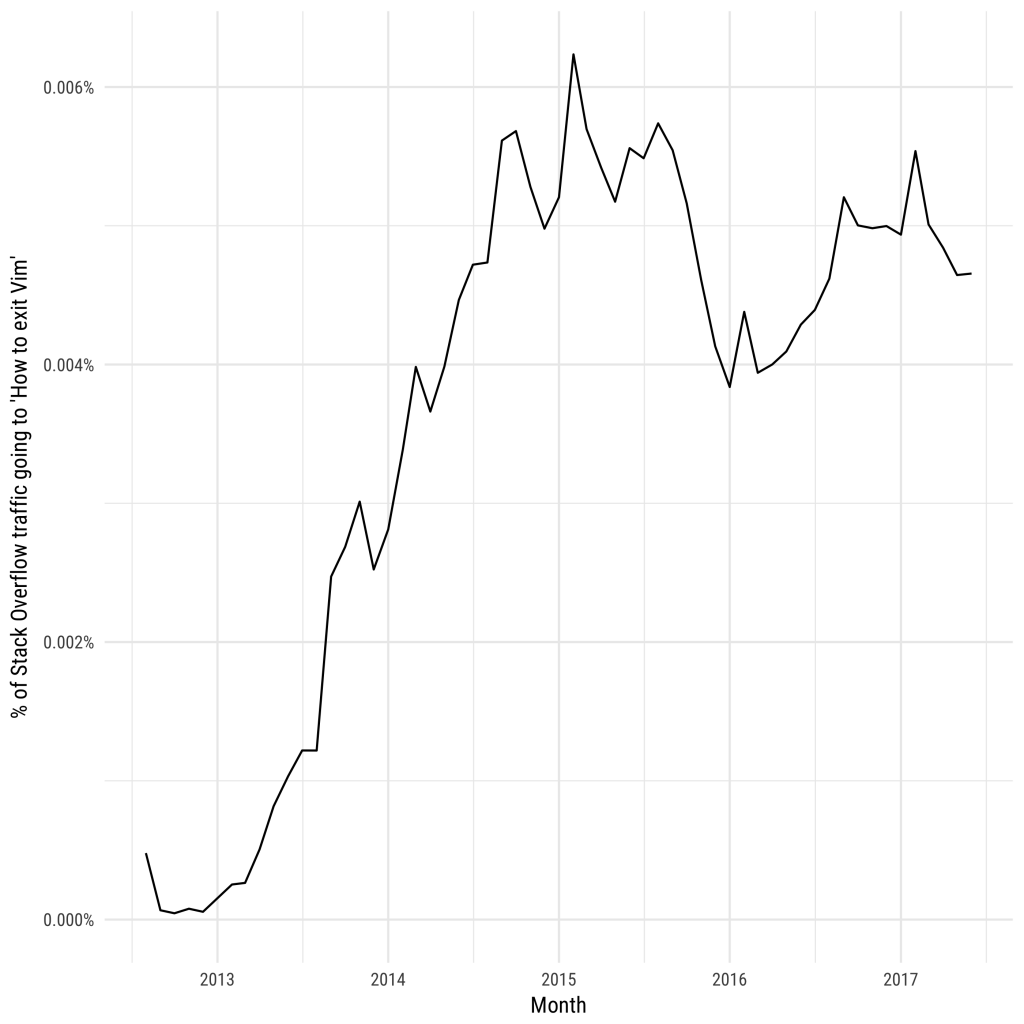
\includegraphics[width=0.4\textwidth]{exiting_vim.png}%
    }%
    \hfill%
    \subfloat{%
        
\includegraphics[width=0.4\textwidth]{vim_meme.jpeg}%
    }%
        \caption{Source: \url{https://stackoverflow.blog/2017/05/23/stack-overflow-helping-one-million-developers-exit-vim/}}
    \end{figure}
\end{frame}

\subsection{Some data}
\begin{frame}{Who uses Vim?}
  \begin{itemize}
    \item Most popular editor in 2006 in Linux Journal readers.
    \item Third most popular editor in 2016 in Stack Overflow
    \item Fifth most popular editor nowadays in Stack Overflow.
    \item 40\% of sysadmins stackoverflow users use Vim.
  \end{itemize}
  \text{Vim is not just for nosaltgic nerds!}
\end{frame}
%------------------------------------------------
\section{Introduction to Vim}
%------------------------------------------------

\subsection{What is Vim} 

\begin{frame}
  \frametitle{What is VIM?}
  Vim is a terminal-based text editor oriented to programmers with highly eficiency writting.
  \begin{figure}
    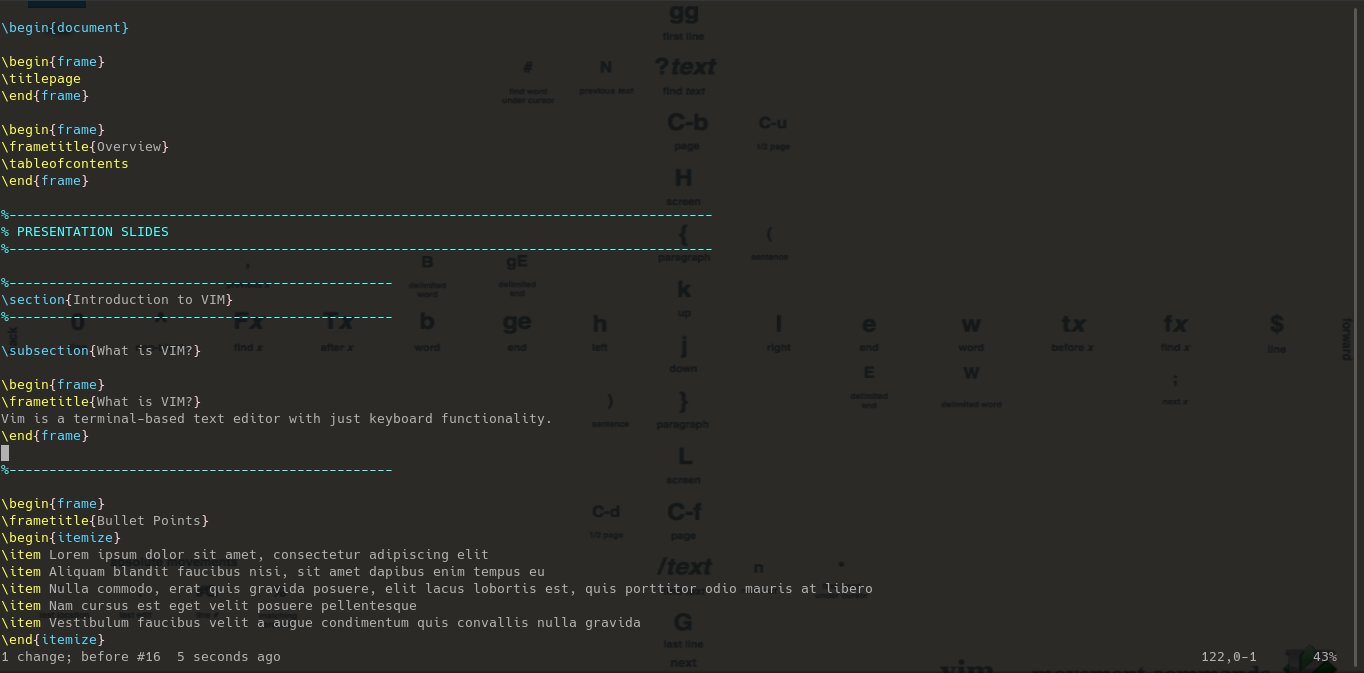
\includegraphics[width=0.8\linewidth]{vimscreenshot.png}
  \end{figure}
\end{frame}

%------------------------------------------------
\subsection{Vim features}
\begin{frame}
  \frametitle{Vim features}
  \begin{itemize}
    \item Keyboard focused.
    \item Text autocompletition 
    \item Terminal multiplexed
    \item More than 200 default key commands.
    \item Highly configurable
    \item Programmer focused
    \item Modes for implementing diferent functions
  \end{itemize}
\end{frame}
%------------------------------------------------
\subsection{Modes}
\begin{frame}
  \frametitle{Modes}
  Vim has 3 main modes with its variations:
  \begin{block}{Insert mode}
    Mainly we will enter this mode with the key i from normal mode. In this mode any character key we pressed will be inserted on the place of the cursor.
  \end{block}
  \begin{block}{Normal mode}
    This is the default mode of vim. When you start up vim you are in this mode. In this mode you can type several commands to change to other modes,move efitienly the cursor, paste, etc..
  \end{block}
  \begin{block}{Visual mode}
    In this mode, wich have several variations you can select text to cut, copy, replace. Its variations consists in the way you select code, for ex: Visual line will be selecting line by line while visual will be selecting character by character.
  \end{block}
  \end{frame}
  %--------------- movement ------------------------
  \section{Moving in Vim}
  \begin{frame}
    \frametitle{Moving in vim (intro)}
  Moving the cursor arround the screen in Normal mode can be performed in many ways. 
  \begin{figure}
      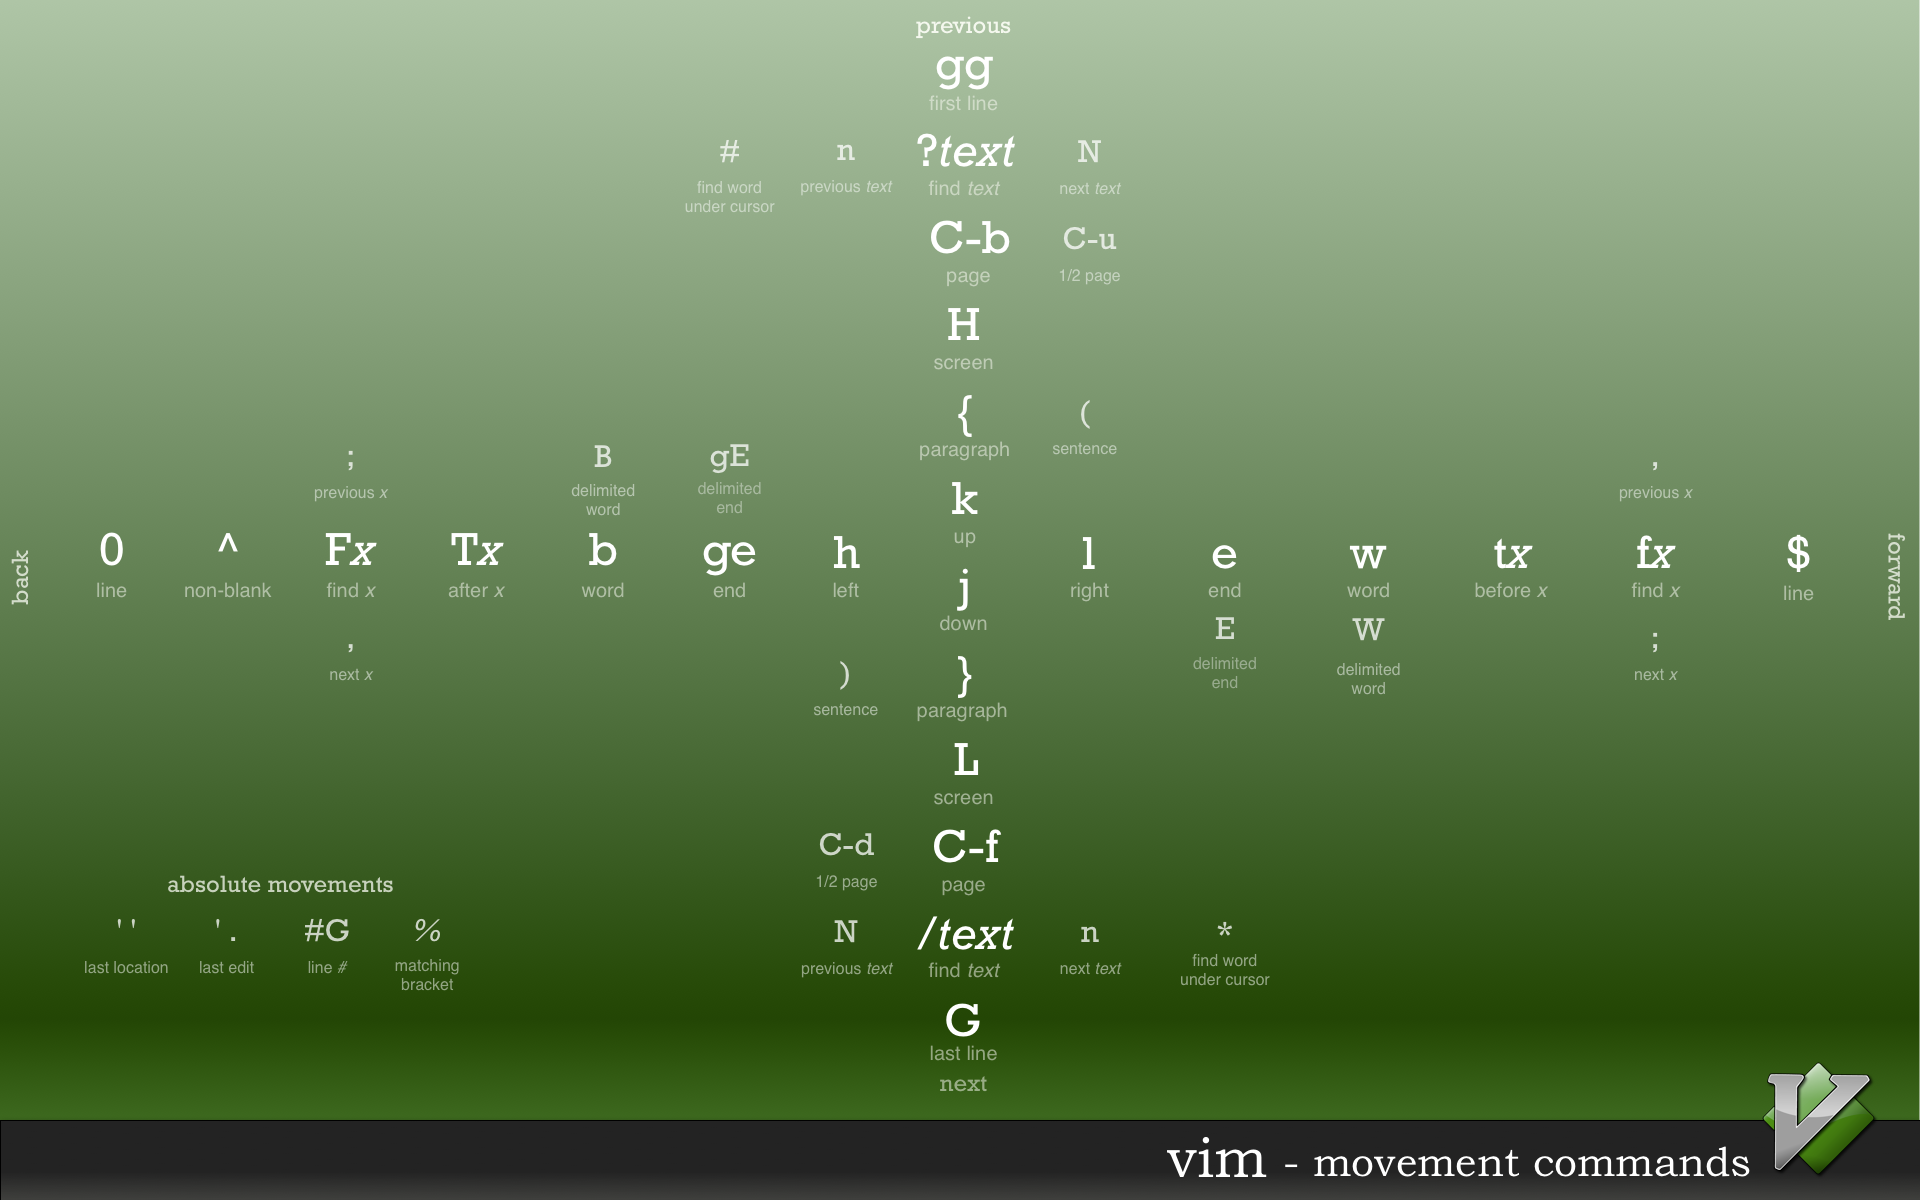
\includegraphics[width=0.8\linewidth]{movement.png}
    \end{figure}
  \end{frame}
  \subsection{Basic moving}
  \begin{frame}{Basic moving}
    \begin{figure}[htp] 
    \centering
    \subfloat[Vim moving]{%
        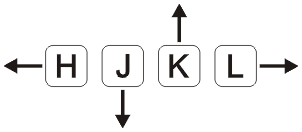
\includegraphics[width=0.4\textwidth]{hjkl_movement.png}%
       
        }%
    VS
    \subfloat[Clasic moving]{%
        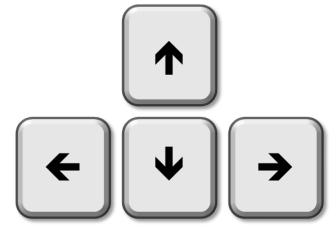
\includegraphics[width=0.4\textwidth]{arrowKeys.png}%
    }%
    \end{figure}
  \end{frame}
  \subsection{Moving keystrokes}
  \begin{frame}{Moving keystrokes(1)}
\begin{center}
\begin{tabular}{ |c|c|c| } 
 \hline
 Command & Explanation \\ \hline
 h j k l & moving arround as arrow keys \\ \hline
 w b & next and last word  \\ \hline
\end{tabular}
\end{center}


      
  \end{frame}
    
\end{document} 
